\documentclass[compress]{beamer}

\usepackage[nofonts]{ctex}
\setCJKmainfont[ItalicFont={Kaiti SC}]{Kaiti SC}%
%\setCJKmainfont[ItalicFont={AR PL KaitiM GB}]{AR PL KaitiM GB}%
%\setCJKsansfont{WenQuanYi Zen Hei}% 文泉驿的黑体

\mode<beamer>
{
    \setbeamercovered{transparent}
    \useinnertheme{rounded}
    \useoutertheme{split}
    \usecolortheme{rose}
    \usecolortheme{seahorse}

    \expandafter\def\expandafter\insertshorttitle\expandafter{%
    \insertshorttitle\hfill%
    \insertframenumber\,/\,\inserttotalframenumber}
}

\mode<handout>
{
	\usetheme{default}
	\usepackage{pgfpages}
	\pgfpagesuselayout{4 on 1}[a4paper,landscape,border shrink=5mm]
}


\usepackage{amsmath,latexsym,amssymb,amsfonts,amsbsy}
\usepackage{graphicx}
\usepackage{hyperref}
\usepackage{listings}
\usepackage{fancyvrb}
\fvset{frame=single,fontsize=\small}

\newcommand{\romannumber}[1]{{\textrm{\uppercase\expandafter{\romannumeral
#1}}}}

\setbeamercolor{dblue}{fg=white,bg=blue!40!black} % for beamercolorbox
\newenvironment{pblock}{\begin{beamercolorbox}[rounded=true,
                  shadow=true]{dblue}}{\end{beamercolorbox}}

\graphicspath{{figure/}}

\lstset{
	basicstyle=\footnotesize\ttfamily, % print whole listing footnotesize
	keywordstyle=\footnotesize\ttfamily\color{black}\bfseries, 
	identifierstyle=\footnotesize\ttfamily\color{blue}, 
	commentstyle=\footnotesize\ttfamily\itshape, 
	stringstyle=\footnotesize\ttfamily,
	frame=single, 
	numbers=left, numberstyle=\tiny,
	stepnumber=1, numbersep=10pt,
	showtabs=false, tabsize=4,
	showstringspaces=false,
	breaklines=true, breakatwhitespace=true,
	language=sh,
}   


%%%%%%%%%%%%%%%%%%%%%%%%%%%%%%%%%%%%%%%%%%%%%%%%%%%%%%%%%%%%%%%%%
%    body                                                       %
%%%%%%%%%%%%%%%%%%%%%%%%%%%%%%%%%%%%%%%%%%%%%%%%%%%%%%%%%%%%%%%%%


\begin{document}

\AtBeginSection[]
{ 
    \begin{frame}<beamer> 
		\frametitle{内容提要} 
		\tableofcontents[currentsection,currentsubsection] 
	\end{frame} 
} 
					
\title{Shell程序设计---2}

\author[\href{http://c.pku.edu.cn/}{http://c.pku.edu.cn/}]
{曹东刚\\\href{mailto:caodg@sei.pku.edu.cn}{caodg@sei.pku.edu.cn}}

\institute{Linux程序设计环境 \\
\href{http://c.pku.edu.cn/}{
http://c.pku.edu.cn/}}

\date{}

\titlegraphic{
\includegraphics[height=0.17\textwidth]{Overlays/logo.pdf}}

\begin{frame}
	\titlepage
\end{frame}

\section{条件判断}

\begin{frame}[fragile]
\frametitle{条件判断}

\begin{Verbatim}
~$ test condition
~$ [ condition ]
\end{Verbatim}

\begin{block}{条件判断} 
判断字符串是否相等, 检查文件状态, 数字测试等.
\begin{itemize}
\item 测试的结果为 true (返回0) 或者 false (返回1),
\item 用 \verb*~[ condition ]~ 的时候要注意, condition 左右两侧必须要有空格
\item 引用变量的时候最好加双引号, 例 \verb~"$arg"~
\item test, true, false 既是 shell 函数, 同时也是 shell 命令.
\end{itemize}
\end{block}
\end{frame}

\begin{frame}[fragile]
  \frametitle{示例}
\begin{Verbatim}
~$ test 1
~$ test 0
~$ test true
~$ test false
~$ [ 1 ]
\end{Verbatim}
\end{frame}

\begin{frame}[fragile]
\frametitle{文件属性判断}

{\footnotesize

\begin{tabular}{|l@{\hspace{0.5cm}}p{6cm}|}
\hline

表达式 & 含义 \\ \hline

\verb=-d file= & file 存在且是目录 \\
\verb=-e file= & file 存在 \\
\verb=-f file= & file 存在且是普通文件  \\
\verb=-r file= & file 存在且可读 \\
\verb=-w file= & file 存在且可写 \\
-x file & file 存在且可执行\\
\verb=-s file= & file 存在且长度非零 \\
\verb=-h file= & file 存在且为符号链接 \\
\verb=file1 -nt file2= & file1 比 file2 新 \\
\verb=file1 -ot file2= & file1 比 file2 旧\\ \hline
\end{tabular}
}
\end{frame}

\begin{frame}[fragile]
  \frametitle{示例}

\noindent\textbf{例: 测试当前目录的文件 check.sh 是否可执行} \\
\begin{Verbatim}
~$ [ -x check.sh ]
~$ echo $?
\end{Verbatim}
\textbf{例: 测试是否存在目录文件 mydir} \\
\begin{Verbatim}
~$ [ -d mydir ]
~$ echo $?
\end{Verbatim}
\end{frame}

\begin{frame}[fragile]
\frametitle{字符串比较}

\begin{tabular}{|l@{\hspace{1cm}}p{6cm}|}
\hline

表达式 & 含义 \\ \hline

\verb~-n str~ & str 长度非0 \\
\verb~-z str~ & str 长度为0 \\
\verb~str1 = str2~ & str1和str2相同\footnote{bash中也可以用==判断字符串相等} \\
\verb~str1 != str2~ & str1和str2不等 \\\hline
\end{tabular}
\end{frame}

\begin{frame}[fragile]
  \frametitle{示例}
\noindent\textbf{例: 字符串str1=\verb~"aa bb"~, 判断是否等于
\verb~"aabb"~}\\
\begin{Verbatim}
~$ [ "$str1" = "aabb" ]
\end{Verbatim}

\noindent\textbf{比较} \\
\begin{Verbatim}
~$ [ $str1 = "aabb" ]
\end{Verbatim}

\noindent\textbf{例: 判断字符串str1和str2是否相等}\\
\begin{Verbatim}
~$ [ "$str1" = "$str2" ]
\end{Verbatim}
\end{frame}

\begin{frame}[fragile]
\frametitle{数字串比较}

\begin{tabular}{|l@{\hspace{1cm}}p{6cm}|}
\hline

表达式 & 含义 \\ \hline

\verb~int1 -eq int2~ & int1和int2相等 \\
\verb~int1 -ne int2~ & int1和int2不等 \\
\verb~int1 -gt int2~ & int1大于int2 \\
\verb~int1 -ge int2~ & int1大于等于int2 \\
\verb~int1 -lt int2~ & int1小于int2 \\
\verb~int1 -le int2~ & int1小于等于int2 \\ \hline
\end{tabular}
\end{frame}

\begin{frame}[fragile]
  \frametitle{示例}

  \noindent\textbf{例: 数字串 int1=\verb~"1234"~, 判断是否等于
  \verb~"01234"~}\\
\begin{Verbatim}
~$ [ "$int1" -eq "01234" ]
\end{Verbatim}

\noindent\textbf{比较} \\
\begin{Verbatim}
~$ [ "01234" = "1234" ]
\end{Verbatim}

\noindent\textbf{例: 判断字符串 str 长度是否大于 3} \\
\begin{Verbatim}
~$ [ `expr length "$str"` -gt 3 ]
~$ [ $(expr length "$str") -gt 3 ]
\end{Verbatim}
\end{frame}

\begin{frame}[fragile]
\frametitle{复合表达式}

{\footnotesize
\begin{tabular}{l@{\hspace{1cm}}l}\hline

\verb~\( expression \)~ & 一组表达式, expression 为真则表达式为真 \\
\verb~! expression~ & expression 为假则表达式为真 \\
\verb~expr1 -a expr2~ & expr1和expr2同时为真则表达式为真 \\
\verb~expr1 -o expr2~ & expr1和expr2有一个为真则表达式为真 \\ \hline

\end{tabular}} \\
\vspace*{0.5cm}
\pause
\begin{Verbatim}
~$ [ -z "$DTHOME" -a -d /usr/dt ]
~$ [ -z "$DTHOME" ] && [ -d /usr/dt ]
\end{Verbatim}

\end{frame}

\section{控制结构}

\begin{frame}[fragile]
\frametitle{命令执行顺序}

Unix提供了多种控制命令执行顺序的机制. 例如,
确保文件成功复制后, 才删除原来的文件.

\begin{itemize}
  \item \alert{;} 顺序执行
  \item \alert{\&\&} 只有 \verb=&&= 左侧执行成功才执行右边命令
  \item \alert{\textbar\textbar}  只有 \verb=||= 左侧执行失败才执行右边命令
\item \alert{\&} 后台执行
\end{itemize}

\end{frame}

\begin{frame}[fragile]
  \frametitle{示例}
  \begin{block}<+-> {先关闭eth0, 再启动eth0 }
\verb#~$ ifconfig eth0 down ; ifconfig eth0 up#
 \end{block}
 \begin{block}<+->{ 先复制目录, 成功后再删除原来目录 }
\verb#~$ cp -r apps ./bak && rm -rf apps#
\end{block}
\begin{block}<+->{ 复制文件, 如果出错则打印 Error }
\verb#~$  cp a.txt b.txt || echo Error#
\end{block}

\begin{block}<+->{ 后台执行fetchmail程序 }
\verb#~$ fetchmail & #
\end{block}

\end{frame}


\begin{frame}[fragile]
  \frametitle{if 语句: 多行模式}
\begin{Verbatim}
if condition1
then
    list1
elif condition2
then
    list2
else
    list3
fi
\end{Verbatim}
\end{frame}

\begin{frame}[fragile]
  \frametitle{if 语句: 单行模式}

\begin{Verbatim}
if condition1; then 
	list1; 
elif condition2; then 
	list2; 
else 
	list3; 
fi;
\end{Verbatim}
\end{frame}

\begin{frame}
\frametitle{注意事项}

常见错误:
\begin{itemize}
\item 单行模式时, then前面漏掉分号";"
\item 使用elif语句时忘记then
\item 用else if 或者 elsif 而不是elif
\item if语句的末尾用了if而不是fi
\end{itemize}

\end{frame}

\begin{frame}[fragile]
\frametitle{示例 1}

\begin{lstlisting}
if uuencode simsun.ttc simsun.ttc > simsun.uu ; then
    echo "Encoded simsun.ttc to simsun.uu"
elif rm simsun.uu ; then
    echo "Encoding failed, temporary files removed."
else
    echo "An error occured."
fi
uuencode simsun.ttc simsun.ttc | mail y@org.cn
uudecode message.eml
\end{lstlisting}
\end{frame}

\begin{frame}[fragile]
\frametitle{示例 2}

\begin{lstlisting}
if [ ! -d $HOME/bin ] ; then
    mkdir $HOME/bin
fi
\end{lstlisting} 
\pause
比较:
\begin{lstlisting}
[ ! -d $HOME/bin ] && mkdir $HOME/bin
\end{lstlisting}
\end{frame}

\begin{frame}[fragile]
\frametitle{case}

case语句的基本语法为
\begin{Verbatim}
case word in
    pattern1)
        list1
        ;;
    pattern2)
        list2
        ;;
esac
\end{Verbatim}
\end{frame}

\begin{frame}
  \frametitle{规则}
\begin{itemize}
\item 字符串word与每一个模式进行比较, 直到找到一个匹配, 然后执行其后的命令清单
\item 若找不到匹配, case语句不执行任何动作并退出
\item 匹配数量无上限, 但至少应有一个
\item 模式可使用与路径名相同的特殊字符, 以及``或''字符 ``\textbar''
\end{itemize}
\end{frame}

\begin{frame}[fragile]
\frametitle{示例 1}

\begin{lstlisting}
case "$TERM" in
    network | dialup | unknown | vt[0-9][0-9][0-9])
        TERM=vt100 ;;
    *term)
        TERM=xterm ;;
    *)
        echo "Error, quit"
        exit 1
        ;;
esac
\end{lstlisting}
\end{frame}

\begin{frame}[fragile]
\frametitle{示例 2}

提示用户输入yes, y, n, No \\
\begin{lstlisting}
echo "Do you wish to continue ? [Yes/No]
read ANS
case "$ANS" in
    y|Y|[yY][eE][sS])
        process ;;
    n|N|[nN][oO])
        abort ;;
    *)
        echo "Error input"
        ;;
esac
\end{lstlisting}
\end{frame}

\begin{frame}[fragile]
\frametitle{for}

for语句的基本语法为\\
\begin{Verbatim}
for name in wordlist ; do
    list
done
\end{Verbatim}

\begin{itemize}
\item name是变量名
\item wordlist是被空格分开的单词序列
\item 每次循环时, name被设为单词中的下一个单词
\end{itemize}
\end{frame}

\begin{frame}[fragile]
\frametitle{示例}

\begin{lstlisting}
for i in 0 1 2 3 4 5 6
do
    echo $i
done

for i in `seq 1 2 100`
do
    echo $i
done
\end{lstlisting}
\end{frame}

\begin{frame}[fragile]
  \frametitle{示例}

\begin{lstlisting}
counter=0
for f in *
do
    counter=`expr $counter + 1`
done
echo "There are $counter files"
\end{lstlisting}
\end{frame}

\begin{frame}[fragile]
\frametitle{while}

while语句的基本语法为\\
{
\begin{Verbatim}

while command ; do
    list
done
\end{Verbatim}
}

\begin{itemize}
\item command是要执行的单条命令, 通常是一个test表达式
\item list称为while 循环体
\item 若 command 的退出状态为0, 则执行 list; 否则退出
\end{itemize}
\end{frame}

\begin{frame}[fragile]
\frametitle{示例 1}

\begin{lstlisting}
x=0
while [ $x -lt 10 ]
do
    echo $x
    x=`echo "$x + 1" | bc`
done
\end{lstlisting}
\end{frame}

\begin{frame}[fragile]
  \frametitle{示例 2: 验证用户的输入}
\begin{lstlisting}
RESPONSE=
while [ -z "$RESPONSE" ]
do
    echo "Enter a directory name "
    read RESPONSE
    if [ ! -d "$RESPONSE" ] ; then
        echo "ERROR: please input a directory name"
        RESPONSE=
    fi
done
\end{lstlisting}
\end{frame}

\begin{frame}[fragile]
\frametitle{select}

select 循环提供了一种从用户可选项中创建编号菜单的便捷形式
\footnote{select由ksh引入, 在bash上兼容, 但bourne sh不支持}. 基本语法为\\
{ \small
\begin{Verbatim}
select name in wordlist ; do
    list
done
\end{Verbatim}
}

\begin{itemize}
\item wordlist是由空格分开的单词序列
\item 用户输入值保存在变量 \$REPLY 中
\item 若没有使用循环控制机制跳出select循环, 则重复选择过程
\end{itemize}
\end{frame}

\begin{frame}[fragile]
\frametitle{示例}

\begin{lstlisting}
select COMPONENT in comp1 comp2 comp3 all none
do
    case $COMPONENT in
    comp1|comp2|comp3) process $COMPONENT ;;
    all) process comp1
        process comp2
        process comp3
        ;;
    none) break ;;
    *) echo "ERROR: Invalid selection, $REPLY." ;;
    esac
done
\end{lstlisting}
\end{frame}

\begin{frame}[fragile]
\frametitle{无限循环和break}

无限循环永远不中止. 例: \\
\begin{lstlisting}
while :
do
    read CMD
    case "$CMD" in
    [qQ]|[qQ][uU][iI][tT]) break ;;
    *) process $CMD ;;
    esac
done
\end{lstlisting}
\end{frame}

\begin{frame}[fragile]
\frametitle{continue命令}

continue命令中止当前迭代, 但不退出整个循环.  例: \\

\begin{lstlisting}
for FILE in FILES
do
    if [ ! -f "$FILE" ] ; then
        echo "ERROR: $FILE is not a file."
        continue
    fi
    # process the file
done
\end{lstlisting}
\end{frame}

\begin{frame}[fragile]
\frametitle{综合示例---打印 usage 语句}

\begin{lstlisting}
USAGE="Usage: `basename $0` [-c|-t] [file|directory]"
case "$1" in
    -t) TARGS="-tvf $2" ;;
    -c) TARGS="-cvf $2.tar $2" ;;
    *)  echo "$USAGE"
        exit 0
        ;;
esac
tar $TARGS
\end{lstlisting}
\end{frame}

\begin{frame}[fragile]
\frametitle{综合示例---检查参数数目}

\begin{lstlisting}
USAGE="Usage: `basename $0` [-c|-t] [file|directory]"
if [ $# -lt 2 ] ; then
    echo "$USAGE"
    exit 1
fi

case "$1" in
    -t) TARGS="-tvf $2" ;;
    -c) TARGS="-cvf $2.tar $2" ;;
    *)  echo "$USAGE"
        exit 0
        ;;
esac
tar $TARGS
\end{lstlisting}
\end{frame}

\begin{frame}[fragile]
\frametitle{综合示例---检查参数语义}
\begin{lstlisting}[lineskip=-0.01pt]
USAGE="Usage: `basename $0` [-c|-t] [file|directory]"
if [ $# -lt 2 ] ; then
    echo "$USAGE"
    exit 1
fi
case "$1" in
    -t) TARGS="-tvf"
        for i in "$@" ; do
            if [ -f "$i" ] ; then tar $TARGS "$i" ; fi ;
        done
        ;;
    -c) TARGS="-cvf $2.tar $2"
        tar $TARGS
        ;;
    *)  echo "$USAGE"
        exit 0 ;;
esac
\end{lstlisting}
\end{frame}

\begin{frame}[fragile]
\frametitle{综合示例---进一步提高}
\begin{lstlisting}[lineskip=-0.01pt]
case "$1" in
    -t) shift ; TARGS="-tvf"
        for i in "$@" ; do
            if [ -f "$i" ] ; then
                FILES=`tar $TARGS "$i" 2>/dev/null`
                if [ $? -eq 0 ] ; then
                    echo ; echo "$i" ; echo "$FILES"
                else
                    echo "ERROR: $i not a tar file."
                fi
            else
                echo "ERROR: $i not a file."
            fi
        done
        ;;
\end{lstlisting}
\end{frame}

\begin{frame}[fragile]
\frametitle{综合示例---进一步提高 (cont.)}

\begin{lstlisting}[firstnumber=last]
    -c) shift ; TARGS="-cvf"
        tar $TARGS archive.tar "$@"
        ;;
    *)  echo "$USAGE"
        exit 0 ;;
esac
\end{lstlisting}
\end{frame}

\begin{frame}
\frametitle{参数选项分析的两种方法}

一种是通过 \alert{case} 语句手工分析, 另一种是通过 \alert{getopts} 命令实现.

\alert{getopts}命令的语法为: getopts option-string variable

\begin{itemize}
\item  option-string 为包含所有单字符选项的字符串, 这些选项应该赋予一个变量, 即 variable
\item 通常使用的 variable 变量名为OPTION
\item {getopts}支持额外参数, 通过在option-string中的选项后面加上``:''字符即可实现.
在这种情况下, 选项被分析后, 额外参数被设置为变量 OPTARG 的值

\end{itemize}

\end{frame}


\begin{frame}
\frametitle{getopts分析过程}
\begin{enumerate}[<+-|alert@+>]
    \item \label{getopts:item1} {getopts} 检查所有参数, 找到以 ``-''字符开头的字符
    \item 将``-''后的字符与option-string中给出的字符比较
    \item \label{getopts:item3} 若找到匹配, 则variable被设置为选项, 否则 variable被设置为 ``?''字符
        \begin{itemize}
            \item 若找到匹配且option-string中的字符后跟``:'', 则读入下一个参数, 将其赋值给 OPTARG
        \end{itemize}
    \item 重复 \ref{getopts:item1} - \ref{getopts:item3}, 直至处理完所有选项
    \item 当分析结束后, {getopts}返回非零值并退出, 并设置变量OPTIND作为下一参数的位置索引
\end{enumerate}
\end{frame}


\begin{frame}[fragile]
\frametitle{getopts示例---问题描述}

\noindent\textbf{写一个脚本uu.sh, 调用uuencode将二进制文件文本化.} \\
\noindent uuencode的调用形式为 uuencode [file] name , 读入文件 file, 将内容编码输出到屏幕.
uu.sh接受如下参数

\begin{itemize}
    \item -f  : 指明输入文件名
    \item -o  : 指明输出文件名
    \item -v  : 指明脚本应输出详细执行信息
\end{itemize}

\noindent \textbf{uu.sh 可能的命令}

\begin{Verbatim}
$ uu.sh chap01.pdf
$ uu.sh -f chap01.pdf -o chap01.uu
\end{Verbatim}

\end{frame}

\begin{frame}[fragile]
\frametitle{getopts示例---读入参数}

\begin{lstlisting}
#!/bin/sh
USAGE="Usage: `basename $0` [-v] [-f file] [-o file]";
VERBOSE=false

while getopts f:o:v OPTION ; do
        case "$OPTION" in
        f) INFILE="$OPTARG" ;;
        o) OUTFILE="$OPTARG" ;;
        v) VERBOSE=true ;;
        \?) echo "$USAGE" ;
                exit 1 ;;
        esac
done
\end{lstlisting}
\end{frame}

\begin{frame}[fragile]
\frametitle{getopts示例---错误处理}

脚本应该检查输入文件, 进行人性化处理\\
\begin{lstlisting}[firstnumber=last]
shift `expr $OPTIND - 1`

if [ -z "$1" -a -z "$INFILE" ] ; then
        echo "ERROR: Input file was not specified."
        exit 1
fi

if [ -z "$INFILE" ] ; then INFILE="$1" ; fi

: ${OUTFILE:=${INFILE}.uu}

\end{lstlisting}
\end{frame}

\begin{frame}[fragile]
\frametitle{getopts示例---任务处理}

\begin{lstlisting}[firstnumber=last]
if [ -f "$INFILE" ] ; then
   if [ "$VERBOSE" = "true" ] ; then
        echo -e "uuencoding $INFILE to $OUTFILE ... \c"
   fi
   uuencode $INFILE $INFILE > $OUTFILE ; RET=$?
   if [ "$VERBOSE" = "true" ] ; then
        MSG="Failed."
        if [ $RET -eq 0 ] ; then MSG="Done." ; fi
        echo $MSG
    fi
else
    echo "ERROR: $INFILE not exists"
fi
\end{lstlisting}
\end{frame}

\section{函数}

\begin{frame}
\frametitle{函数定义}

shell函数的正式定义为:\\
name() { list ; }

\begin{itemize}
\item 函数将一个名字name与命令清单list绑定在一起
\item 函数定义时必须要用到``(''和``)''字符
\item shell函数可以替代二进制文件或shell内置同名命令
\item 函数在当前shell执行
\item 可以用shell模拟alias命令
\end{itemize}


\end{frame}

\begin{frame}[fragile]
\frametitle{函数示例---无参}

\noindent \textbf{例: 模拟csh的source命令}\\[1ex]
\begin{lstlisting}
source() { . "$@" ;}
\end{lstlisting}

\pause
\noindent \textbf{例: 打印当前PATH的值} \\
\begin{lstlisting}
lspath() {
    OLDIFS="$IFS"
    IFS=:
    for DIR in $PATH ; do echo $DIR ; done
    IFS=$OLDIFS
}
\end{lstlisting}
\end{frame}

\begin{frame}[fragile]
\frametitle{函数示例---传递参数}

\begin{lstlisting}
SetPath() {
    for _DIR in "$@"
    do
        if [ -d "$_DIR" ] ; then
            PATH="$PATH":"$_DIR"
        fi
    done
    export PATH
    unset _DIR
}
\end{lstlisting}
\end{frame}

\section{信号处理}

\begin{frame}
\frametitle{信号处理}

\begin{itemize}
\item 信号(signal)是向一个程序发出的软件中断, 它指出发生了一个重要的事件
\item 可利用信号户要求程序做不属于正常流程的事情
\end{itemize}

{\small
\begin{tabular}{p{2cm}p{2cm}p{5cm}}\hline
Num & Name & Action\\ \hline
1 & HUP & 重起进程 \\
2 & INT & 中断 \\
3 & QUIT & 退出 \\
9 & KILL & 强制杀死(unblock)\\
15 & TERM & 软中止 \\ \hline
\end{tabular}
}
\end{frame}

\begin{frame}
\frametitle{信号缺省动作}

每个信号都有一个与之关联的缺省动作: 在接收到该信号时执行的动作.
可能的缺省动作有:

\begin{itemize}
\item 中止进程
\item 忽略信号
\item 内核转储
\item 停止进程
\item 继续一个停止的进程, 等
\end{itemize}
\end{frame}

\begin{frame}
\frametitle{处理信号}

一个脚本或程序可以用三种方式处理信号:

\begin{itemize}
\item 不做任何处理而让缺省动作发生
\item 忽略信号并继续执行
\item 捕获信号并执行一些信号特定命令
\end{itemize}

\end{frame}

\begin{frame}
  \frametitle{捕获信号}

\alert{trap} 命令设置或取消接收到一个信号时的动作, 其语法为\\
trap function signals

\begin{itemize}
\item 若不给出function, 则将给定信号的动作重设为缺省动作
\item \alert{trap}常用于清除临时文件, 忽略信号, 设置计时器等
\end{itemize}
\end{frame}

\begin{frame}[fragile]
\frametitle{示例: 清除临时文件}

\begin{lstlisting}
trap "rm -f $TEMP ; exit 2" 1 2 3 15
\end{lstlisting}
\pause 
\textbf{更复杂的清除} \\
\begin{lstlisting}
CleanUp() {
    if [ -f "$OUTFILE" ] ; then
        printf "Cleanning up ..."
        rm -f "$OUTFILE" 2> /dev/null
        echo "Done."
    fi
}
trap CleanUp 1 2 3 15
\end{lstlisting}
\end{frame}

\begin{frame}[fragile]
\frametitle{忽略信号}

\noindent \verb~trap '' 1 2 3 15~ \\
\pause
\noindent 或者 \\
\noindent \verb~trap : 1 2 3 15~ \\
\pause
\noindent 在关键操作期间忽略信号 \\

\begin{lstlisting}
trap '' 1 2 3 15
DoImportantStuff
trap 1 2 3 15
\end{lstlisting}
\end{frame}

\begin{frame}
\frametitle{定时器技术}
有时候, 程序对多任务进行批处理. 为了防止某个任务非正常运行, 占有处理器不退出(如死循环, 等待其它进程的信号),需要
一种机制及时终止该任务. 定时器技术可以解决此类问题.
\begin{itemize}
\item 通常需要三个进程: 控制主进程, 定时器进程, 任务子进程
\item 各进程之间通过信号机制通信
\end{itemize}
\end{frame}

\begin{frame}
\frametitle{原理}
子任务正常返回\\[2ex]
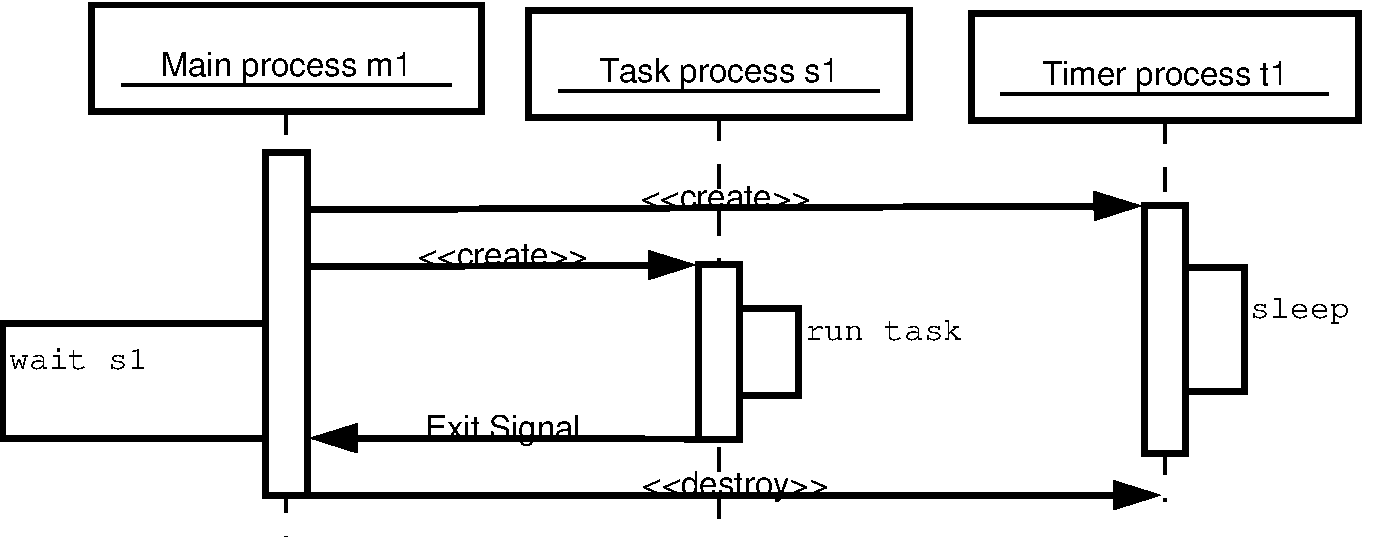
\includegraphics[width=1.0\hsize]{success.pdf}
\end{frame}

\begin{frame}
\frametitle{原理}
子任务阻塞, 定时器进程触发Alarm 信号\\[2ex]
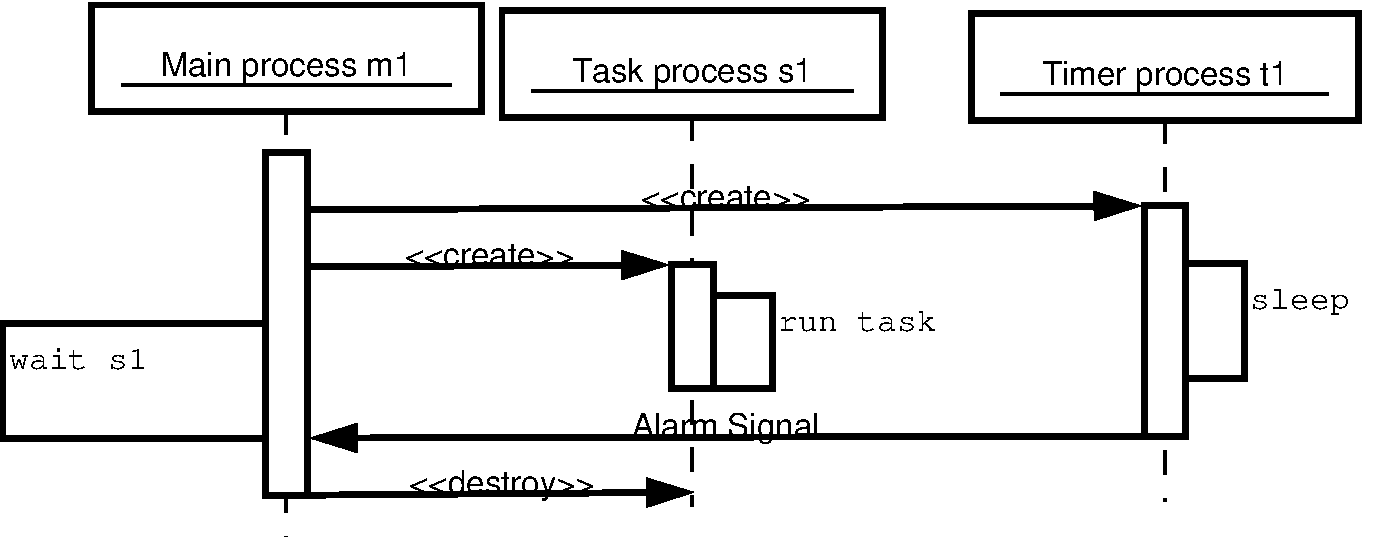
\includegraphics[width=1.0\hsize]{trap.pdf}
\end{frame}

\begin{frame}[fragile]
  \frametitle{代码示例: 信号处理函数}

\begin{lstlisting}
AlarmHandler()
{
    echo "Got SIGALARM, cmd took too long"
    kill ${CHPROCIDS:-$!}
    if [ $? -eq 0 ] ; then
        TIMERPROC=
        echo "Sub process killed."
    fi
}
\end{lstlisting}
\end{frame}

\begin{frame}[fragile]
  \frametitle{代码示例: 设置定时器}

\begin{lstlisting}[firstnumber=last,lineskip=-0.01pt]
setTimer()
{
    DEF_TOUT=${1:-10};
    if [ $DEF_TOUT -ne 0 ] ; then
        sleep $DEF_TOUT && kill -s 14 $$ &
        echo "settimer $!"
        TIMERPROC=$!
    fi
}

UnsetTimer()
{
    CHPROCIDS=
    [ -n "$TIMERPROC" ] && kill $TIMERPROC
}
\end{lstlisting}
\end{frame}

\begin{frame}[fragile]
  \frametitle{代码示例: 主进程}

\begin{lstlisting}[firstnumber=last]
trap AlarmHandler 14

if [ -f date.sh ] ; then
    echo " -->   run date.sh "
    setTimer 3
    sh date.sh &
    CHPROCIDS="$CHPROCIDS $!"
    wait $!
    echo " -->   end date.sh "
    UnsetTimer
fi
wait
\end{lstlisting}

\end{frame}

\end{document}
